\chapter{I moduli in esame e i dati che producono}
\label{chap:moduli}

Questo capitolo descrive i moduli sensore impiegati nel lavoro sperimentale, analizzandone le specifiche tecniche, le interfacce di comunicazione e i dati che forniscono. L'analisi permette di comprendere quali grandezze ciascun modulo mette effettivamente a disposizione e con quali limiti, e costituisce la base su cui sono state costruite la piattaforma di acquisizione e le analisi dei capitoli successivi.

Il capitolo è organizzato come segue. La Sezione~\ref{sec:c3-1} presenta il radar \ldb{}, il modulo principale della tesi, con le specifiche, la piedinatura, gli strumenti di configurazione, il protocollo seriale, la engineering mode che sblocca i dati per gate e l'identità dell'esemplare in prova. La Sezione~\ref{sec:c3-2} presenta con la stessa struttura il secondo radar, l'\ldc{}. La Sezione~\ref{sec:c3-3} descrive il PIR \pir{} e la configurazione adottata. La Sezione~\ref{sec:c3-4} illustra la piattaforma di acquisizione, dal repository di riferimento ai firmware, al formato dei dati e alla catena di analisi. La Sezione~\ref{sec:c3-5} verifica i dati prodotti e descrive i comportamenti del modulo da tenere presenti nel leggere i risultati. La Sezione~\ref{sec:c3-6} spiega perché le soglie dell'\ldb{} sono rimaste di fabbrica mentre l'\ldc{} ha richiesto una taratura.

\FloatBarrier
\section{Il radar \ldb{}}
\label{sec:c3-1}

L'\ldb{} è un modulo radar a 24~GHz per il rilevamento della presenza umana prodotto da Shenzhen Hi-Link Electronic \cite{hilinkManualV104}. Si presenta come una piccola scheda che integra il chip radar FMCW, le antenne a patch per trasmissione e ricezione, un microcontrollore che elabora il segnale e, nella variante B, un ricetrasmettitore Bluetooth per la configurazione da smartphone. L'elaborazione del segnale avviene interamente a bordo. Il modulo emette il segnale, analizza l'eco e comunica all'esterno soltanto il risultato, cioè lo stato di presenza, la distanza e l'energia del bersaglio, attraverso un connettore a cinque piedini che porta una linea seriale e un'uscita digitale. È in grado di distinguere un bersaglio in movimento da uno stazionario e di mantenere la presenza anche su una persona immobile, sfruttando i micro-movimenti del corpo descritti nella Sezione~\ref{subsec:corpo-immobile}. Il modulo è mostrato nella Figura~\ref{fig:c3-foto2410}.

\begin{figure}[!htb]
\centering
\includegraphics[width=0.7\linewidth]{Foto_LD2410B}
\caption{Il modulo \ldb{}, retro (in alto) e fronte (in basso). Sul fronte le due antenne a patch alle estremità e il chip radar al centro; sul retro il connettore a cinque piedini, il microcontrollore e i quarzi. Immagine tratta da \cite{studiopietersLD2410}.}
\label{fig:c3-foto2410}
\end{figure}

\subsection{Specifiche tecniche}
\label{sec:c3-1-1}

Le specifiche dichiarate dal produttore sono riassunte nella Tabella~\ref{tab:c3-1} \cite{hilinkManualV104,hilinkManualV103,ld2410bDatasheet}.

\begin{table}[!htb]
\centering
\caption{Specifiche dell'\ldb{} \cite{hilinkManualV104,hilinkManualV103,ld2410bDatasheet}.}
\label{tab:c3-1}
\small
\begin{tabularx}{\linewidth}{@{}lX@{}}
\toprule
\textbf{Parametro} & \textbf{Valore} \\
\midrule
Frequenza di lavoro & 24–24,25~GHz, banda ISM \\
Tecnologia & FMCW (onda continua modulata in frequenza) \\
Portata dichiarata & 5–6~m \\
Campo visivo & \(\pm\)60\(^\circ\) \\
Alimentazione & 5~V, alimentatore con capacità \(>\)~200~mA \\
Corrente media & 80~mA \\
Interfaccia & UART 256000~baud, 8N1 \\
Bluetooth & integrato (variante B), password di default HiLink \\
Dimensioni & circa 35~mm \(\times\) 7~mm \\
Gate di distanza & 9 (0–8) \\
Risoluzione gate & 0,75~m oppure 0,20~m \\
\bottomrule
\end{tabularx}
\end{table}

\subsection{Piedinatura e collegamento all'ESP32}
\label{sec:c3-1-2}

Il modulo espone cinque piedini, definiti nella Tabella 1 del datasheet \cite{ld2410bDatasheet}. La Tabella~\ref{tab:c3-2} riporta la funzione di ciascuno e il collegamento all'ESP32 adottato in questo lavoro. Come d'uso per una linea seriale, i due fili sono incrociati, cioè il piedino di trasmissione del radar va al piedino di ricezione dell'ESP32 e viceversa.

\begin{table}[!htb]
\centering
\caption{Piedinatura dell'\ldb{} (Tabella 1 del datasheet \cite{ld2410bDatasheet}) e collegamento all'ESP32.}
\label{tab:c3-2}
\small
\begin{tabularx}{\linewidth}{@{}clXl@{}}
\toprule
\textbf{Pin} & \textbf{Nome} & \textbf{Funzione} & \textbf{Collegamento ESP32} \\
\midrule
1 & OUT & presenza digitale (alto = persona) & non collegato \\
2 & UART\_Tx & il radar trasmette & GPIO25 (RX2) \\
3 & UART\_Rx & il radar riceve & GPIO26 (TX2) \\
4 & GND & massa & GND \\
5 & VCC & alimentazione & VIN (5~V) \\
\bottomrule
\end{tabularx}
\end{table}

Il piedino OUT, che riporta lo stato di presenza come semplice livello logico, non è stato collegato perché la stessa informazione è già contenuta nel frame seriale, come verificato nella Sezione~\ref{sec:c3-5-4}.

La velocità di 256000~baud richiede una delle UART hardware dell'ESP32. Si è usata la seconda, sui pin GPIO25 e GPIO26, perché la prima è occupata dal collegamento USB con il PC.

\subsection{Strumenti di configurazione}
\label{sec:c3-1-3}

Il produttore distribuisce due strumenti di configurazione:

\begin{itemize}
  \item il LD2410 Tool per PC, che dialoga con il modulo via UART attraverso un adattatore USB-seriale \cite{hilinkDriveLD2410B}
  \item l'applicazione mobile HLKRadarTool, che si collega via Bluetooth con la password di default HiLink \cite{hilinkV244}.
\end{itemize}

Entrambi permettono di leggere e modificare i parametri (gate massimi, soglie per gate, timeout di presenza, risoluzione), di attivare l’engineering mode e di osservare in tempo reale i grafici dell'energia per gate e la distanza rilevata. L'applicazione mobile offre in più l'auto-calibrazione delle soglie introdotta dal firmware V2.44, non utilizzata in questo lavoro. Inizialmente il LD2410 Tool è stato utilizzato per una prima verifica del modulo e per confrontare i dati acquisiti. In seguito si è fatto fede alla lettura via UART, perché lo strumento mostra per le sensibilità il valore 100 su tutti i gate, mentre il comando di lettura del protocollo restituisce la scala di fabbrica riportata nella Tabella~\ref{tab:c3-6}, coerente con il comportamento osservato. Lo strumento non mostra la versione del firmware e non offre funzioni di aggiornamento. La Figura~\ref{fig:c3-tool2410} mostra la schermata dello strumento con il modulo in prova.

\begin{figure}[!htb]
\centering
\includegraphics[width=0.85\linewidth]{Tool_LD2410B}
\caption{Schermata del LD2410 Tool collegato all'esemplare in prova, in engineering mode. A sinistra i parametri letti dal modulo, con le sensibilità mostrate a 100 su tutti i gate; al centro le energie per gate della componente in movimento e di quella stazionaria (in colore) con le soglie di fabbrica sovrapposte (in verde); in basso la distanza rilevata negli ultimi due minuti.}
\label{fig:c3-tool2410}
\end{figure}

\subsection{Protocollo seriale}
\label{sec:c3-1-4}

Il protocollo seriale prevede due tipi di frame per lo scambio di informazioni fra il modulo e l'host \cite{hilinkProtoV107}:

\textbf{Frame di comando} (inviati dall'host al modulo): La struttura è riportata nella Tabella~\ref{tab:c3-3}. Ogni comando va inviato dentro la modalità di configurazione, durante la quale il modulo sospende l'invio dei dati. Il modulo risponde con un frame della stessa struttura, in cui la parola di comando ha il bit più significativo posto a uno ed è seguita da uno stato (zero = successo) e dagli eventuali dati di risposta. Tutti i campi a più byte sono little-endian.

\begin{table}[!htb]
\centering
\caption{Struttura del frame di comando, dall'host al modulo \cite{hilinkProtoV107}.}
\label{tab:c3-3}
\small
\begin{tabularx}{\linewidth}{@{}llX@{}}
\toprule
\textbf{Campo} & \textbf{Lunghezza} & \textbf{Valore} \\
\midrule
Intestazione & 4~byte & FD FC FB FA \\
Lunghezza dati & 2~byte & little-endian \\
Parola di comando & 2~byte & little-endian \\
Valore del comando & variabile & dipende dal comando \\
Chiusura & 4~byte & 04 03 02 01 \\
\bottomrule
\end{tabularx}
\end{table}

\textbf{Frame di dati} (inviati dal modulo all'host a cadenza fissa): La struttura è riportata nella Tabella~\ref{tab:c3-4}. Il byte di tipo distingue il frame normale (0x02) da quello di engineering mode (0x01), e il byte di stato è una maschera di bit in cui un bersaglio in movimento e uno stazionario possono essere presenti insieme. I campi aggiunti dall'engineering mode sono quelli che fanno la differenza fra un sensore binario e uno strumento di misura (Sezione~\ref{sec:c3-1-5}).

\begin{table}[!htb]
\centering
\caption{Struttura del frame di dati, dal modulo all'host \cite{hilinkProtoV107}.}
\label{tab:c3-4}
\small
\begin{tabularx}{\linewidth}{@{}lcX@{}}
\toprule
\textbf{Campo} & \textbf{Lunghezza} & \textbf{Valore} \\
\midrule
Intestazione & 4~byte & F4 F3 F2 F1 \\
Lunghezza dati & 2~byte & little-endian \\
Tipo di dato & 1~byte & 0x01 = engineering mode, 0x02 = normale \\
Testa & 1~byte & 0xAA \\
Stato del bersaglio & 1~byte & maschera: 0x01 in movimento, 0x02 stazionario \\
Distanza in movimento & 2~byte & cm, little-endian \\
Energia in movimento & 1~byte & 0–100 \\
Distanza stazionaria & 2~byte & cm, little-endian \\
Energia stazionaria & 1~byte & 0–100 \\
Distanza di rilevamento & 2~byte & cm, little-endian \\
\multicolumn{3}{@{}l@{}}{\emph{(solo in engineering mode)}} \\
Gate massimo movimento & 1~byte &  \\
Gate massimo stazionario & 1~byte &  \\
Energie per gate, movimento & 9~byte & gate 0–8, valori 0–100 \\
Energie per gate, stazionario & 9~byte & gate 0–8, valori 0–100 \\
Sensore di luce & 1~byte & 0–255 \\
Stato del pin OUT & 1~byte &  \\
\multicolumn{3}{@{}l@{}}{\emph{(fine della parte engineering)}} \\
Coda & 1~byte & 0x55 \\
Controllo & 1~byte & 0x00 \\
Chiusura & 4~byte & F8 F7 F6 F5 \\
\bottomrule
\end{tabularx}
\end{table}

I comandi utilizzati in questo lavoro sono riassunti nella Tabella~\ref{tab:c3-5}:

\begin{table}[!htb]
\centering
\caption{Comandi del protocollo seriale utilizzati in questo lavoro \cite{hilinkProtoV107}.}
\label{tab:c3-5}
\small
\begin{tabularx}{\linewidth}{@{}lX@{}}
\toprule
\textbf{Comando} & \textbf{Funzione} \\
\midrule
0x00FF & entra in modalità configurazione \\
0x00FE & esce dalla modalità configurazione \\
0x0062 & attiva engineering mode \\
0x0063 & disattiva engineering mode \\
0x00A0 & legge la versione firmware \\
0x00A5 & legge il MAC Bluetooth \\
0x0061 & legge i parametri correnti (soglie, gate, timeout) \\
0x0060 & imposta i parametri \\
0x00AA & imposta la risoluzione di distanza \\
0x000B & auto-calibrazione del rumore di fondo (firmware V2.44) \\
\bottomrule
\end{tabularx}
\end{table}

\subsection{Engineering mode e dati per gate}
\label{sec:c3-1-5}

In modalità normale il modulo riporta, per ogni frame, lo stato di presenza, la distanza e l'energia del bersaglio in movimento e stazionario, cioè una decisione già presa accompagnata da pochi valori aggregati. In engineering mode aggiunge le energie di ciascuno dei nove gate, separatamente per la componente in movimento e per quella stazionaria (diciotto valori aggiuntivi) più la lettura del fotosensore e lo stato del pin OUT.

Le serie temporali di questi canali sono la materia prima di tutte le analisi quantitative dei capitoli successivi, e per questo il firmware realizzato tiene l’engineering mode sempre attiva.

\subsection{Identità dell'esemplare in prova}
\label{sec:c3-1-6}

Per la riproducibilità dei risultati, la Tabella~\ref{tab:c3-6} riporta identità e parametri dell'esemplare effettivamente usato, letti via UART con i comandi di lettura della Tabella~\ref{tab:c3-5}.

\begin{table}[!htb]
\centering
\caption{Identità e parametri dell'esemplare di \ldb{} in prova, letti via UART.}
\label{tab:c3-6}
\small
\begin{tabularx}{\linewidth}{@{}lX@{}}
\toprule
\textbf{Dato} & \textbf{Valore letto} \\
\midrule
Versione firmware & 2.44.25070917 \\
Versione protocollo & 1 \\
MAC Bluetooth & 5E:E4:93:22:B9:3F \\
Baud confermato & 256000, 8N1 \\
Risoluzione gate & 75~cm; gate 0–8; portata configurabile 600~cm (8 gate \(\times\) 0,75~m \cite[§5.2]{hilinkManualV104}) \\
Timeout di presenza (no-one duration) & 5~s \\
Soglie di movimento (gate 0–8) & 50, 50, 40, 30, 20, 15, 15, 15, 15 \\
Soglie stazionarie (gate 0–8) & 0, 0, 40, 40, 30, 30, 20, 20, 20 \\
\bottomrule
\end{tabularx}
\end{table}

Le soglie coincidono valore per valore con quelle di fabbrica riportate nella Tabella 7 del protocollo \cite{hilinkProtoV107}. Le soglie stazionarie dei gate 0 e 1 sono indicate dal documento come non impostabili, con le conseguenze discusse nella Sezione~\ref{sec:c3-5-2}. Il firmware 2.44 è l'ultima versione rilasciata dal produttore, la stessa che introduce l'auto-calibrazione citata nella Sezione~\ref{sec:c3-1-3} \cite{hilinkV244}.

\FloatBarrier
\section{Il radar \ldc{}}
\label{sec:c3-2}

L'\ldc{} è un modulo radar a 24~GHz per il rilevamento della presenza umana, anch'esso prodotto da Shenzhen Hi-Link Electronic \cite{hilinkManualLD2420}. È una scheda quadrata che integra il chip radar FMCW, le antenne e un microcontrollore, ma non dispone di Bluetooth, quindi la configurazione avviene soltanto via seriale. L'elaborazione è a bordo e verso l'esterno il modulo espone, su un connettore a cinque piedini, una linea seriale e un'uscita digitale di presenza. Riporta lo stato di occupazione e la distanza del bersaglio in movimento. Sulla persona immobile, invece, mantiene la presenza sfruttando i micro-movimenti del corpo (Sezione~\ref{subsec:corpo-immobile}), ma non è in grado di misurarne la distanza, come dichiarato dal produttore \cite[§8]{hilinkManualLD2420}. Il modulo è mostrato nella Figura~\ref{fig:c3-foto2420}.

\begin{figure}[!htb]
\centering
\begin{minipage}[t]{0.42\linewidth}\centering\includegraphics[width=\linewidth]{LD2420_fronte}\end{minipage}\hfill
\begin{minipage}[t]{0.42\linewidth}\centering\includegraphics[width=\linewidth]{LD2420_retro}\end{minipage}
\caption{Il modulo \ldc{}, fronte e retro. Sul fronte le antenne a patch e il connettore J2 a cinque piedini usato per alimentazione e seriale; sul retro il microcontrollore e il connettore J1 dell'interfaccia di programmazione, non utilizzato. Immagini del produttore \cite[Tab.~3-1 e 3-2]{hilinkManualLD2420}.}
\label{fig:c3-foto2420}
\end{figure}

\subsection{Specifiche tecniche}
\label{sec:c3-2-1}

Le specifiche dichiarate dal produttore sono riassunte nella Tabella~\ref{tab:c3-7} \cite{hilinkManualLD2420}.

\begin{table}[!htb]
\centering
\caption{Specifiche dell'\ldc{} secondo il manuale del produttore \cite{hilinkManualLD2420}.}
\label{tab:c3-7}
\small
\begin{tabularx}{\linewidth}{@{}lX@{}}
\toprule
\textbf{Parametro} & \textbf{Valore} \\
\midrule
Frequenza di lavoro & 24–24,25~GHz, banda di sweep 0,25~GHz \\
Tecnologia & FMCW (onda continua modulata in frequenza) \\
Potenza irradiata (EIRP) & 11~dBm \\
Portata dichiarata & a parete: 8~m su bersaglio in movimento, 6~m su micro-movimento; a soffitto: 5~m e 4~m \\
Distanza minima & 0,2~m, nessuna zona morta \\
Accuratezza di distanza & \(\pm\)0,35~m (valore teorico, dipende dalla corporatura del bersaglio) \\
Campo visivo & \(\pm\)60\(^\circ\) (§1.1); \(\pm\)45\(^\circ\) in orizzontale e in elevazione (§5.2) \\
Cadenza dati & 10~Hz \\
Alimentazione & 3,0–3,6~V, tipica 3,3~V \\
Corrente media & 50~mA \\
Interfaccia & UART 115200~baud, 8N1 \\
Bluetooth & assente \\
Dimensioni & 20 \(\times\) 20~mm \\
Temperatura operativa & \(-\)40 / +85~\(^\circ\)C \\
Gate di distanza & 16 (0–15) \\
Risoluzione gate & 0,70~m, fissa \\
\bottomrule
\end{tabularx}
\end{table}

\textbf{Due incongruenze nella documentazione ufficiale:}

\begin{itemize}
  \item Apertura angolare: il manuale la riporta con valori diversi in due punti, \(\pm\)60\(^\circ\) fra le caratteristiche principali e \(\pm\)45\(^\circ\) nella sezione sul montaggio a parete \cite[§1.1 e §5.2]{hilinkManualLD2420}.
  \item Ritardo di scomparsa del bersaglio: il manuale indica l’intervallo 0--65\,535 \cite[§4.2.1]{hilinkManualLD2420}, mentre il documento di protocollo indica 0x00–0x0F \cite[Tab. 2]{hilinkProtoLD2420}. Proprio gli esempi contenuti nel protocollo, però, usano i valori 30 e 26, che cadono fuori da quell'intervallo.
\end{itemize}

\subsection{Piedinatura e collegamento all'ESP32}
\label{sec:c3-2-2}

Il modulo espone cinque piedini, definiti nella Tabella 3-2 del manuale \cite{hilinkManualLD2420}. La Tabella~\ref{tab:c3-8} riporta la funzione di ciascuno e il collegamento all'ESP32 adottato in questo lavoro.

\begin{table}[!htb]
\centering
\caption{Piedinatura del connettore J2 dell'\ldc{} \cite[Tab. 3-2]{hilinkManualLD2420} e collegamento all'ESP32.}
\label{tab:c3-8}
\small
\begin{tabularx}{\linewidth}{@{}llXl@{}}
\toprule
\textbf{Pin} & \textbf{Nome} & \textbf{Funzione} & \textbf{Collegamento ESP32} \\
\midrule
J2-1 & 3V3 & alimentazione 3,0–3,6~V & 3V3 \\
J2-2 & GND & massa & GND \\
J2-3 & OT1 & UART\_TX, 0–3,3~V (il radar trasmette) & GPIO16 (RX) \\
J2-4 & RX & UART\_RX, 0–3,3~V (il radar riceve) & GPIO17 (TX) \\
J2-5 & OT2 & uscita di presenza: alto occupato, basso libero & non collegato \\
\bottomrule
\end{tabularx}
\end{table}

La documentazione del componente ESPHome \cite{esphomeLD2420} segnala che nei moduli con firmware precedente alla versione 1.5.3 la trasmissione seriale avviene sul piedino OT2 anziché su OT1 e a 256000~baud anziché 115200. Il firmware dell'esemplare in dotazione è la 1.6.1, quindi più recente, e infatti il modulo trasmette su OT1 a 115200~baud, mentre OT2 riporta lo stato di presenza come livello logico, come da manuale.

\subsection{Strumenti di configurazione}
\label{sec:c3-2-3}

Il produttore distribuisce l'\ldc{}\_TOOL per PC \cite{hilinkDriveLD2420}, che dialoga con il modulo via UART attraverso un adattatore USB-seriale. Permette di leggere e scrivere i parametri (gate minimo e massimo, ritardo di scomparsa e le trentadue soglie per gate), di osservare in tempo reale l'energia di ciascun gate e la distanza rilevata, e di salvare la configurazione in un file XML. Le soglie sono mostrate in decibel, cioè come \(10\cdot\log_{10}\) del valore intero che il modulo usa internamente. La Figura~\ref{fig:c3-tool2420} mostra la schermata dei parametri con la configurazione di fabbrica dell'esemplare.

\begin{figure}[!htb]
\centering
\includegraphics[width=0.85\linewidth]{Tool_LD2420}
\caption{Schermata dei parametri dell'\ldc{}\_TOOL collegato all'esemplare in prova, con la configurazione di fabbrica letta dal modulo: gate massimo 12, ritardo di scomparsa 30~s, le sedici soglie di attivazione e le sedici di mantenimento in decibel, versione firmware 1.6.1.}
\label{fig:c3-tool2420}
\end{figure}

La funzione più importante è la scansione del rumore di fondo (bottom noise scan, \cite[§4.2.2–4.2.3]{hilinkManualLD2420}). A stanza vuota il tool registra per ogni gate il livello di energia del fondo e ne ricava le due soglie, una di attivazione (trigger, consigliata a circa 5 volte il rumore) e una di mantenimento (maintain, a 2–5 volte), che poi scrive nella memoria non volatile del modulo.

\subsection{Protocollo seriale}
\label{sec:c3-2-4}

Il documento di protocollo \cite{hilinkProtoLD2420} descrive esclusivamente i comandi di configurazione, con frame delimitati dall'intestazione FD FC FB FA e dalla chiusura 04 03 02 01 e con lunghezza e parola di comando a 2~byte little-endian. I comandi disponibili sono riassunti nella Tabella~\ref{tab:c3-9}, e i parametri si leggono e si scrivono per identificatore.

\begin{table}[!htb]
\centering
\caption{Comandi e identificatori di parametro del protocollo dell'\ldc{} \cite{hilinkProtoLD2420}. Il comando segnato con l'asterisco non compare nel protocollo ufficiale ed è ricostruito dalla comunità ESPHome \cite{esphomeLD2420src}.}
\label{tab:c3-9}
\small
\begin{tabularx}{\linewidth}{@{}lX@{}}
\toprule
\textbf{Comando} & \textbf{Funzione} \\
\midrule
0x00FF & entra in modalità comandi \\
0x00FE & esce dalla modalità comandi \\
0x0000 & legge la versione firmware \\
0x0068 & riavvia il modulo \\
0x0008 & legge parametri (per identificatore) \\
0x0007 & scrive parametri (per identificatore) \\
0x0012* & scrive un parametro di sistema: valore 0x0004 per l'energy mode, 0x0064 per la modalità di testo di fabbrica \\
id 0x00 / 0x01 & gate minimo / gate massimo (0–15) \\
id 0x04 & ritardo di scomparsa del bersaglio, in secondi \\
id 0x10–0x1F & soglie di attivazione (trigger) dei gate 0–15 \\
id 0x20–0x2F & soglie di mantenimento (maintain) dei gate 0–15 \\
\bottomrule
\end{tabularx}
\end{table}

\textbf{Dati trasmessi dal modulo:} Il documento di protocollo descrive soltanto i comandi che il modulo riceve e non il formato con cui trasmette i risultati del rilevamento. Il manuale indica di aprire un terminale seriale a 115200~baud per leggerli \cite[§4.1]{hilinkManualLD2420}. In modalità di fabbrica il modulo trasmette righe di testo che riportano la presenza rilevata (ON), l'assenza di presenza (OFF) e la distanza del bersaglio (Range NN).

L'unità di misura del campo Range non è indicata in nessuno dei due documenti del produttore. Le prove a distanza nota descritte nel Capitolo~\ref{chap:confronto} hanno mostrato che il valore è espresso in centimetri quando un bersaglio è presente, mentre in assenza di bersaglio il campo assume un valore di riposo compreso fra 0 e 6, privo di significato come distanza. Il valore si aggiorna di rado e va quindi letto soltanto quando la presenza è alta.

\textbf{Persistenza dei parametri.} I parametri scritti con il comando 0x0007 sono accettati e riletti correttamente, ma il modulo li perde al ciclo di alimentazione, e il protocollo non prevede un comando di salvataggio. La configurazione di riferimento è quindi quella scritta in memoria non volatile dal tool (Sezione~\ref{sec:c3-2-3}).

\subsection{Energy mode e dati per gate}
\label{sec:c3-2-5}

L'\ldc{} può trasmettere, al posto della sola decisione di presenza, il profilo di energia per gate da cui quella decisione è ricavata. Questa modalità, detta energy mode, non è descritta in alcun documento ufficiale, anche se il tool del produttore la utilizza per tracciare i grafici dell'energia per gate. Il suo funzionamento è stato ricostruito dalla comunità ESPHome tramite reverse engineering, e il risultato è implementato nel componente ld2420 \cite{esphomeLD2420src}, che costituisce la fonte su cui si basa il logger realizzato per questo lavoro. Si attiva con il comando 0x0012 della Tabella~\ref{tab:c3-9}, dopodiché il modulo emette a 10~Hz frame binari da 45~byte con la struttura della Tabella~\ref{tab:c3-10}.

\begin{table}[!htb]
\centering
\caption{Struttura del frame di dati in energy mode, ricostruita dal componente ESPHome \cite{esphomeLD2420src}.}
\label{tab:c3-10}
\small
\begin{tabularx}{\linewidth}{@{}llX@{}}
\toprule
\textbf{Campo} & \textbf{Lunghezza} & \textbf{Valore} \\
\midrule
Intestazione & 4~byte & F4 F3 F2 F1 \\
Lunghezza dati & 2~byte & little-endian \\
Presenza & 1~byte & 0 = libero, 1 = occupato \\
Distanza & 2~byte & cm, little-endian \\
Energie per gate & 16 \(\times\) 2~byte & gate 0–15, interi 0--65\,535, little-endian \\
Chiusura & 4~byte & F8 F7 F6 F5 \\
\bottomrule
\end{tabularx}
\end{table}

Le energie sono interi a 16~bit e, convertite in decibel con la stessa relazione delle soglie, coincidono con i valori mostrati dal tool, a conferma che la struttura ricostruita è corretta.

\subsection{Identità dell'esemplare in prova}
\label{sec:c3-2-6}

La Tabella~\ref{tab:c3-11} riporta identità e parametri dell'esemplare effettivamente usato, letti via UART con i comandi della Tabella~\ref{tab:c3-9} e confrontati con il file XML salvato dal tool.

\begin{table}[!htb]
\centering
\caption{Identità e parametri dell'esemplare di \ldc{} in prova, letti via UART.}
\label{tab:c3-11}
\small
\begin{tabularx}{\linewidth}{@{}lX@{}}
\toprule
\textbf{Dato} & \textbf{Valore letto} \\
\midrule
Versione firmware & 1.6.1 (ultima rilasciata dal produttore) \\
Baud confermato & 115200, 8N1 \\
Gate minimo / massimo impostati & 0 / 12 (minimo / massimo), su un intervallo ammesso 0–15 (portata configurata 840~cm) \\
Ritardo di scomparsa & 30~s \\
Soglie trigger, gate 0–3 & 60\,000, 30\,000, 3000, 2000 (47,8 / 44,8 / 34,8 / 33,0~dB) \\
Soglie maintain, gate 9–15 & 100 (20~dB) \\
\bottomrule
\end{tabularx}
\end{table}

Il modulo era in configurazione di fabbrica \cite{hilinkProtoLD2420}. Il produttore non distribuisce aggiornamenti del firmware, per cui la versione riportata è quella con cui il modulo è stato prodotto.

Il radar in dotazione è con ogni probabilità difettoso, perché nelle prove a distanza nota rileva una persona in movimento fino a circa 1~m e la mantiene fino a 2~m, contro gli 8~m dichiarati. Le energie per gate indicano un trasmettitore molto più debole del previsto, mentre il ricevitore funziona. Soglie, configurazione dei gate, firmware, parser, orientamento e cablaggio sono stati esclusi con prove dedicate. Le conseguenze sul protocollo della campagna sono dichiarate nella Sezione~\ref{sec:protocollo-ld2420}.

\FloatBarrier
\section{Il sensore PIR in dotazione: \pir{}}
\label{sec:c3-3}

Il modulo in dotazione è un \pir{}, il PIR più diffuso per microcontrollori. Sulla scheda si trova l'elemento piroelettrico, coperto dalla cupola bianca della lente di Fresnel (Sezione~\ref{subsec:fresnel}). Il circuito integrato BISS0001 \cite{biss0001} amplifica il segnale e lo trasforma in un'uscita digitale con soglia e tempo di ritenuta. Un regolatore lineare HT7133 porta l'alimentazione a 3,3~V e fissa a questo livello anche l'uscita. Due trimmer regolano la sensibilità, e quindi la portata, e il tempo di ritenuta dell'uscita, mentre un ponticello a tre pin seleziona la modalità di trigger, singolo o ripetibile. Il modulo è mostrato nella Figura~\ref{fig:c3-fotopir}.

\begin{figure}[!htb]
\centering
\includegraphics[width=0.5\linewidth]{Foto_HCSR501}
\caption{Il modulo \pir{}, fronte e retro. Sul fronte la cupola della lente di Fresnel; sul retro il circuito integrato BISS0001, i due trimmer di sensibilità e di ritenuta, il regolatore di tensione, il ponticello di trigger (in giallo) e i tre piedini di uscita. Immagine del distributore \cite{alibabaHCSR501}.}
\label{fig:c3-fotopir}
\end{figure}

\subsection{Specifiche tecniche}
\label{sec:c3-3-1}

Le specifiche dichiarate dal datasheet \cite{hcsr501} sono riassunte nella Tabella~\ref{tab:c3-12}.

\begin{table}[!htb]
\centering
\caption{Specifiche del PIR \pir{} in dotazione (datasheet \cite{hcsr501}).}
\label{tab:c3-12}
\small
\begin{tabularx}{\linewidth}{@{}lX@{}}
\toprule
\textbf{Parametro} & \textbf{Valore} \\
\midrule
Base & BISS0001 + elemento LHI778 \\
Alimentazione & 4,5–20~V DC (collegato a VIN 5~V dell'ESP32) \\
Livello logico di uscita & alto 3,3~V / basso 0~V, grazie al regolatore HT7133 a bordo: compatibile con i GPIO dell'ESP32 senza adattamento \\
Corrente di riposo & \(<\)~50~\textmu{}A \\
Portata & 3–7~m, regolabile con il trimmer di sensibilità \\
Angolo di copertura & cono \(<\)~100\(^\circ\) \\
Tempo di ritenuta & regolabile, 5--200~s dichiarati (circa 3,4~s misurati al minimo del trimmer) \\
Block time & 2,5~s dopo ogni rilascio \\
Trigger & jumper: L = singolo, H = ripetibile \\
Temperatura operativa & \(-\)15 / +70~\(^\circ\)C \\
Dimensioni & 32 \(\times\) 24~mm \\
\bottomrule
\end{tabularx}
\end{table}

\subsection{Piedinatura e collegamento all'ESP32}
\label{sec:c3-3-2}

Il modulo espone tre piedini, riportati nella Tabella~\ref{tab:c3-13} insieme al collegamento all'ESP32 adottato in questo lavoro.

\begin{table}[!htb]
\centering
\caption{Piedinatura dell'\pir{} (visto dal lato dei trimmer) e collegamento all'ESP32.}
\label{tab:c3-13}
\small
\begin{tabularx}{\linewidth}{@{}clXl@{}}
\toprule
\textbf{Pin} & \textbf{Nome} & \textbf{Funzione} & \textbf{Collegamento ESP32} \\
\midrule
1 & GND & massa & GND \\
2 & OUT & uscita di presenza, alto 3,3~V / basso 0~V & GPIO34 \\
3 & VCC & alimentazione 4,5–20~V & VIN (5~V) \\
\bottomrule
\end{tabularx}
\end{table}

\subsection{Configurazione adottata}
\label{sec:c3-3-3}

La configurazione del modulo è riassunta nell'elenco seguente, e i suoi effetti sono discussi nel Capitolo~\ref{chap:confronto}.

\begin{enumerate}
  \item \textbf{Ponticello di trigger}: Le prime acquisizioni sono state svolte in posizione L, poi il ponticello è stato spostato su H ripetendo gli scenari interessati.
  \item \textbf{Trimmer del tempo di ritenuta al minimo}: La ritenuta misurata è di circa 3,4~s, invariata per tutta la campagna.
  \item \textbf{Trimmer di sensibilità a metà corsa:} È stato portato al massimo soltanto nelle prove di portata massima, per verificare il valore dichiarato dal datasheet.
\end{enumerate}

\FloatBarrier
\section{La piattaforma di acquisizione}
\label{sec:c3-4}

I tre sensori sono letti da un'unica piattaforma, costruita perché ogni misura dei capitoli successivi sia riproducibile. La Tabella~\ref{tab:c3-14} elenca i firmware per l'ESP32 e la Tabella~\ref{tab:c3-14b} il software per il PC, diviso in acquisizione, analisi e materiali derivati.

Le sezioni che seguono descrivono il punto di partenza (Sezione~\ref{sec:c3-4-1}), i firmware (Sezione~\ref{sec:c3-4-2}), il formato dei dati che li accomuna (Sezione~\ref{sec:c3-4-3}), lo script di acquisizione (Sezione~\ref{sec:c3-4-4}) e la catena di analisi (Sezione~\ref{sec:c3-4-5}). Tutto il software è nel repository della tesi insieme ai file CSV della campagna, che sono l'unico contenuto non ricostruibile.

\begin{table}[!htb]
\centering
\caption{Il firmware realizzato per l'ESP32. I percorsi sono relativi alla radice del repository.}
\label{tab:c3-14}
\small
\begin{tabularx}{\linewidth}{@{}>{\raggedright\arraybackslash}p{4.3cm}>{\raggedright\arraybackslash}X@{}}
\toprule
\textbf{Sketch} & \textbf{Contenuto} \\
\midrule
firmware/ld2410b\_\allowbreak{}logger & logger CSV a 5~Hz dell'\ldb{} con engineering mode e lettura del PIR (fasi 1--7 della campagna) \\
firmware/ld2420\_\allowbreak{}logger\_\allowbreak{}bin & logger dell'\ldc{} in energy mode, 16 energie a 16~bit, stesso schema CSV \\
firmware/ld2410b\_\allowbreak{}web & web UI della Sezione~\ref{sec:webui}, stesso CSV del logger sulla seriale (Fase 8 della campagna) \\
firmware/test00\_\allowbreak{}ld2410\_\allowbreak{}info,\allowbreak{} test04\_\allowbreak{}set\_\allowbreak{}gate & lettura dei parametri dell'\ldb{} via UART e configurazione del gate massimo \\
firmware/test06\_\allowbreak{}ld2420\_\allowbreak{}set\_\allowbreak{}gate & lettura e scrittura dei parametri dell'\ldc{} via UART (32 soglie, gate, ritardo) \\
firmware/test01\_\allowbreak{}ld2410\_\allowbreak{}base,\allowbreak{} test03\_\allowbreak{}pir\_\allowbreak{}base & sketch diagnostici, baud rate del radar e durata degli impulsi del PIR \\
\bottomrule
\end{tabularx}
\end{table}

\begin{table}[!htb]
\centering
\caption{Il software realizzato per il PC: acquisizione, analisi e materiali derivati. I percorsi sono relativi alla radice del repository.}
\label{tab:c3-14b}
\small
\begin{tabularx}{\linewidth}{@{}>{\raggedright\arraybackslash}p{4.3cm}>{\raggedright\arraybackslash}X@{}}
\toprule
\textbf{Componente} & \textbf{Contenuto} \\
\midrule
HLK-LD2410x/acquire.py & acquisizione dalla seriale con metadati sperimentali, adattato dal repository di riferimento \\
HLK-LD2410x/data & i CSV della campagna e il registro delle sessioni \\
analisi/verifica\_\allowbreak{}engineering.py & controllo di qualità di un CSV prima dell'uso \\
analisi/analizza\_\allowbreak{}test.py & metriche di confronto e aggregazione per scenario \\
analisi/analizza\_\allowbreak{}respiro.py & analisi in frequenza e ricerca del canale migliore \\
analisi/vitalita\_\allowbreak{}proto.py,\allowbreak{} verifica\_\allowbreak{}vitalita\_\allowbreak{}bordo.py & prototipo dell'indice di vitalità e verifica del porting (Capitolo~\ref{chap:vitalita}) \\
analisi/rigenera\_\allowbreak{}tutto.py e script collegati & figure, foglio Excel e pagina di riepilogo, rigenerabili dai CSV con un comando \\
\bottomrule
\end{tabularx}
\end{table}

\subsection{Il repository di riferimento}
\label{sec:c3-4-1}

Il lavoro parte dal repository del relatore \cite{repoCallisto}, che contiene un firmware PlatformIO per ESP32 basato sulla libreria ncmreynolds/ld2410 e uno script Python di acquisizione. Il firmware legge il radar via UART, gestisce opzionalmente un display OLED e un PIR e stampa righe CSV sulla seriale. Lo script acquire.py le salva su file e aggiunge i metadati sperimentali passati da riga di comando. Lo studio del codice ha evidenziato tre limiti per gli scopi di questa tesi:

\begin{enumerate}
  \item \textbf{Campionamento a 1~Hz}, troppo lento per misurare le latenze e insufficiente per l'analisi del respiro, perché il limite di Nyquist a 0,5~Hz coincide con il bordo superiore della banda respiratoria (Sezione~\ref{sec:respiro}).
  \item \textbf{Assenza dell'engineering mode}, quindi viene registrata la sola energia del bersaglio e non i diciotto valori per gate della Sezione~\ref{sec:c3-1-5}.
  \item \textbf{Piedinatura diversa} (radar TX su GPIO17 e RX su GPIO16), quindi i due firmware non sono interscambiabili senza ricablare.
\end{enumerate}

\subsection{I firmware}
\label{sec:c3-4-2}

Per ciascun radar sono stati scritti due programmi per l'ESP32, uno sketch di configurazione che legge e scrive i parametri del modulo e un logger che acquisisce i dati. I due si caricano in momenti diversi. Prima si carica lo sketch, per portare il radar nella configurazione voluta, poi il logger, che resta a bordo per tutta la sessione. Il logger legge il radar e il PIR e stampa sulla porta seriale USB una riga di testo per campione, nel formato della Sezione~\ref{sec:c3-4-3}. L'ESP32 non salva nulla, perché il file viene scritto dallo script di acquisizione sul PC (Sezione~\ref{sec:c3-4-4}). Tutti i programmi stampano all'avvio una riga con il numero di build, così l'esito di una prova non può essere attribuito a un binario diverso da quello caricato. Il collegamento dei tre sensori all'ESP32 è riassunto nella Figura~\ref{fig:c3-collegamenti}.

\begin{figure}[!htb]
\centering
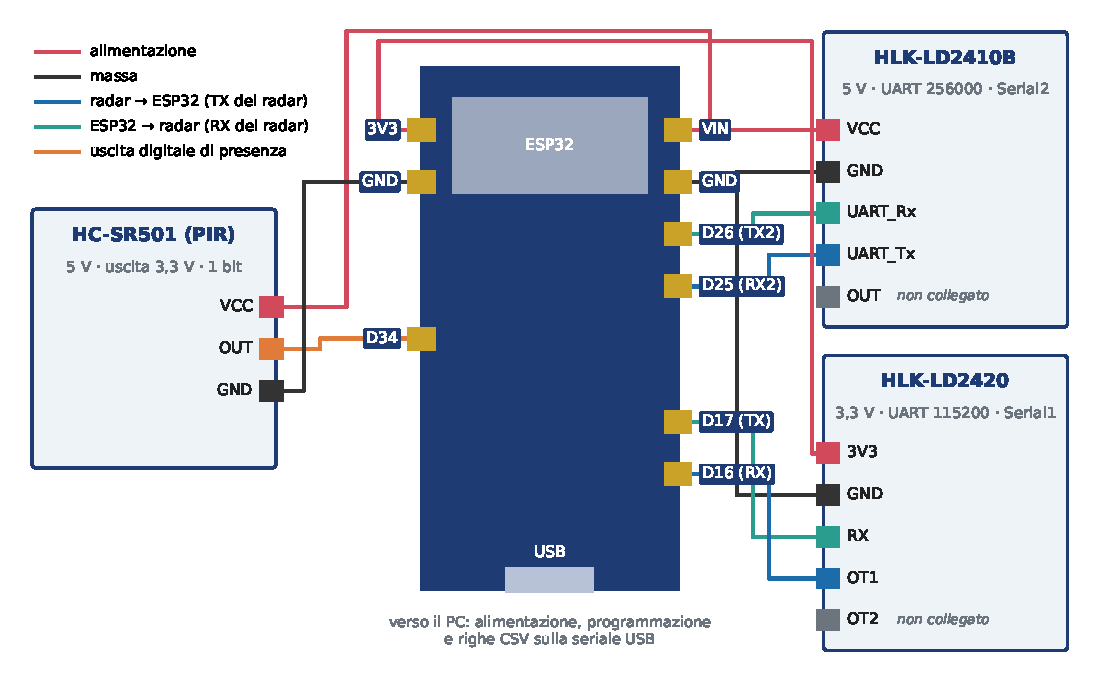
\includegraphics[width=\linewidth]{figures/fig28_collegamenti}
\caption{Collegamento dei tre sensori all'ESP32. L'\ldb{} è alimentato a 5~V da VIN e dialoga sulla seconda UART hardware (GPIO25 e 26); l'\ldc{} è alimentato a 3,3~V e usa una terza UART sui GPIO16 e 17, mentre la sua uscita di presenza OT2 non è collegata perché la presenza arriva dal frame seriale; il PIR è alimentato a 5~V e la sua uscita a 3,3~V va a GPIO34. I due fili della seriale sono incrociati. Le Tabelle~\ref{tab:c3-2}, \ref{tab:c3-8} e \ref{tab:c3-13} riportano il dettaglio dei piedini.}
\label{fig:c3-collegamenti}
\end{figure}

\paragraph{Gli sketch di configurazione}

I due sketch, uno per modulo, hanno tre accorgimenti importanti:

\begin{itemize}
  \item Dopo ogni scrittura i parametri sono riletti per conferma.
  \item Lo sketch avvisa quando la configurazione corrente è diversa da quella di fabbrica, per non condurre acquisizioni con parametri modificati inconsapevolmente.
  \item Nello sketch dell'\ldb{} un comando riscrive i valori di fabbrica dell'esemplare (Tabella~\ref{tab:c3-6}), così da poter tornare in ogni momento alla configurazione di riferimento.
\end{itemize}

Sul \ldc{} lo sketch ha permesso di verificare che le 32 soglie in flash coincidessero con quelle mostrate in decibel dallo strumento del produttore (Sezione~\ref{sec:c3-2-3}).

\paragraph{Il logger dell'\ldb{}}

Il logger dell'\ldb{} usa la libreria MyLD2410 \cite{myld2410}. Tre scelte condizionano la qualità dei dati.

\begin{itemize}
  \item \textbf{Campionamento a 5~Hz a periodo fisso}: il ciclo principale calcola l'istante del campione successivo anziché attendere un intervallo dopo l'elaborazione. Per questo la cadenza misurata è di 200~ms esatti su tutti gli intervalli (Sezione~\ref{sec:c3-5}).
  \item \textbf{Engineering mode attivato all'avvio e verificato}: il firmware entra in configurazione, attiva la modalità, esce e controlla che i frame ricevuti siano del tipo esteso, segnalando l'esito sulla seriale. Un fallimento silenzioso produrrebbe file senza colonne per gate, scoperti solo in analisi.
  \item \textbf{Lettura del PIR}: avviene nello stesso frame, immediatamente prima di comporre la riga CSV, così che i due sensori condividano la base dei tempi per costruzione e non per allineamento a posteriori.
\end{itemize}

\paragraph{Il logger dell'\ldc{}}

Legge i frame da 45~byte dell'energy mode (Sezione~\ref{sec:c3-2-5}) a 10~Hz e li riduce a 5~Hz per coerenza con il resto della campagna. Gate massimo, gate minimo e ritardo di scomparsa possono essere scritti via UART a ogni accensione, ma la scrittura non è persistente (Sezione~\ref{sec:c3-2-4}). Il valore riletto finisce in un commento in testa al CSV, così ogni file dichiara la configurazione con cui è stato acquisito. Il formato delle colonne è nella Sezione~\ref{sec:c3-4-3}.

\paragraph{Il firmware della web UI}

Legge lo stesso radar e lo stesso PIR del logger dell'\ldb{} e scrive sulla seriale le sue stesse colonne, così lo script di acquisizione può girare in parallelo alla pagina. In più pubblica i dati in rete e calcola a bordo l'indice di vitalità (Sezione~\ref{sec:webui}).

\subsection{Il formato dei dati}
\label{sec:c3-4-3}

Tutti i file della tesi seguono lo stesso schema a strati (Tabella~\ref{tab:c3-15}). Le prime nove colonne coincidono con quelle del repository di riferimento e sono prodotte da tutti i firmware. Su queste lavora lo script di confronto del Capitolo~\ref{chap:confronto}, quindi le metriche di presenza, falsi positivi, latenze e distanza si calcolano allo stesso modo per i due radar. Seguono le colonne proprie di ciascun radar, con nomi distinti (menergy, senergy contro energy2420) perché le scale sono diverse, 0--100 contro 0--65\,535, e nessuno script deve confonderle. Le grandezze che un radar non possiede valgono zero. Il solo CSV esportato dalla web UI aggiunge in coda due colonne con il valore e la classe dell'indice di vitalità calcolato a bordo (Capitolo~\ref{chap:vitalita}), messe in fondo perché la catena di analisi non le richiede e le ignora.

\begin{table}[!htb]
\centering
\caption{Schema a strati dei file CSV della tesi. Le prime nove colonne sono comuni a tutti i firmware; le colonne proprie di ciascun radar hanno nomi distinti perché le scale sono diverse.}
\label{tab:c3-15}
\small
\begin{tabularx}{\linewidth}{@{}>{\raggedright\arraybackslash}p{2.1cm}>{\raggedright\arraybackslash}X>{\raggedright\arraybackslash}p{2.4cm}c@{}}
\toprule
\textbf{Strato} & \textbf{Colonne} & \textbf{Prodotte da} & \textbf{N.} \\
\midrule
Base comuni & timestamp\_\allowbreak{}ms, radar\_\allowbreak{}presence, moving\_\allowbreak{}target, stationary\_\allowbreak{}target, moving\_\allowbreak{}distance\_\allowbreak{}cm, stationary\_\allowbreak{}distance\_\allowbreak{}cm, moving\_\allowbreak{}energy, stationary\_\allowbreak{}energy, pir\_\allowbreak{}presence & tutti i firmware & 9 \\
LD2410B & menergy\_\allowbreak{}gate0..8, senergy\_\allowbreak{}gate0..8, light\_\allowbreak{}level, out\_\allowbreak{}level & logger LD2410B, web UI & 20 (29 in totale) \\
LD2420 & energy2420\_\allowbreak{}gate0..15, frames\_\allowbreak{}ok, dist\_\allowbreak{}raw\_\allowbreak{}cm & logger LD2420 & 18 (27 in totale) \\
Metadati & pc\_\allowbreak{}time\_\allowbreak{}s, group\_\allowbreak{}id, trial\_\allowbreak{}id, scenario, ground\_\allowbreak{}truth\_\allowbreak{}presence, ground\_\allowbreak{}truth\_\allowbreak{}state & acquire.py & 6 \\
Indice a bordo & vitality\_\allowbreak{}onboard, vitality\_\allowbreak{}class\_\allowbreak{}onboard & export della web UI (Sezione~\ref{sec:webui}) & 2 \\
\bottomrule
\end{tabularx}
\end{table}

Nei test dell'\ldc{} il PIR non è cablato. Un piedino non collegato leggerebbe zero per tutto il file, e gli script ne ricaverebbero un 100~\% di falsi negativi con una persona davanti. Per questo il firmware scrive il valore sentinella \(-\)1, che lo script di analisi riconosce. In quel caso lo script omette ogni metrica del PIR e lo segnala in una colonna di stato del foglio Excel.

L'intestazione è stampata dal firmware una sola volta all'avvio. Le righe che iniziano con il cancelletto sono commenti, che lo script di acquisizione scarta, e contengono il marcatore di build di ogni sketch e la configurazione dell'\ldc{} (Sezione~\ref{sec:c3-4-2}). Lo script di acquisizione ricostruisce un'intestazione mancante dal numero di colonne (Sezione~\ref{sec:c3-4-4}), ma a 27 colonne il logger dell'\ldc{} e l'engineering mode senza fotosensore non si distinguono, quindi l'intestazione stampata dal firmware è indispensabile.

\subsection{Lo script di acquisizione}
\label{sec:c3-4-4}

Lo script acquire.py legge la seriale e aggiunge a ogni riga le sei colonne di metadati sperimentali della Tabella~\ref{tab:c3-15}, dichiarati dall'operatore da riga di comando. Il file prende il nome dello scenario e del trial, e lo script richiede la sola libreria pyserial.

Lo script ricostruisce l'intestazione dal numero di colonne della prima riga di dati (9 per la modalità base, 29 per l'engineering mode completo), invece di attendere quella stampata dall'ESP32 all'avvio. Altrimenti, quando il reset all'apertura della porta seriale non scatta, il CSV resterebbe vuoto senza alcun avviso.

Per facilitare i test sono stati introdotti:

\begin{itemize}
  \item Un segnale acustico all'istante dell'evento per le misure di latenza (Sezione~\ref{sec:latenza})
  \item Annunci vocali a istanti prefissati per le prove di portata.
\end{itemize}

Entrambi contano dalla prima riga di dati ricevuta, evitando l'errore di 2--3~s che un cronometro esterno introdurrebbe per il reset dell'ESP32.

\subsection{La catena di analisi}
\label{sec:c3-4-5}

L'analisi è svolta da cinque script Python basati sulla sola libreria standard, con l'eccezione di NumPy per la parte in frequenza, più un gruppo di script che produce i materiali derivati e richiede matplotlib, openpyxl e pillow.

\paragraph{verifica\_engineering.py}

È il controllo di qualità di un CSV prima dell'uso. Verifica la cadenza reale e il jitter, presenza delle colonne per gate, percentuale di saturazione a 100 per canale, coerenza fra gate di picco e distanza riportata, rumore di fondo per gate a stanza vuota e transizioni di presenza. Va eseguito a ogni sessione ed è ciò che ha permesso di individuare i comportamenti descritti nella Sezione~\ref{sec:c3-5}.

\paragraph{analizza\_test.py}

Produce i valori su cui si basano i confronti del Capitolo~\ref{chap:confronto}. Su ogni trial calcola falsi positivi in eventi all'ora, falsi negativi in percentuale, latenza di rilevamento e di rilascio con la convenzione dell'evento a istante noto, e statistiche di distanza ed energia. Lo script riunisce le ripetizioni di ogni scenario e per ciascuna metrica riporta la media e la deviazione standard fra i trial. Prima del calcolo scarta i secondi iniziali in cui il soggetto raggiunge la posizione, con una durata che dipende dallo scenario (Sezione~\ref{sec:metriche-transitorio}). Lo script legge indifferentemente i file dei due radar e della web UI.

\paragraph{analizza\_respiro.py}

Esegue l'analisi in frequenza (Sezione~\ref{sec:respiro}) e richiede NumPy. Applica la FFT alla serie di energia, cerca il picco in banda 0,1--0,5~Hz, stima gli atti al minuto ed esporta lo spettro. La modalità di scansione prova tutti i canali di energia, scarta quelli saturi e quelli piatti, li ordina per rapporto segnale-rumore e riporta la mediana delle stime concordi. È nata dal primo pilota del respiro, in cui il canale predefinito, l'energia stazionaria aggregata, era saturo per tutto il file mentre il respiro era leggibile su un gate di movimento. Da allora la ricerca automatica del canale migliore, con criterio dichiarato, è parte del metodo.

\paragraph{vitalita\_proto.py}

È il prototipo dell'indice di vitalità (Capitolo~\ref{chap:vitalita}). Legge i CSV dell'\ldb{} e calcola l'indice campione per campione, sottraendo il fondo per gate, prendendo l'energia del gate in cui il radar riporta il bersaglio e filtrandola con due medie mobili esponenziali. Su un insieme di trial produce la distribuzione dell'indice per scenario e la matrice di confusione delle tre classi, con cui le soglie sono state tarate e poi validate su trial separati. Lo script verifica\_vitalita\_bordo.py ha verificato che il firmware calcoli lo stesso indice del prototipo, confrontando campione per campione le due colonne in coda al CSV della web UI con il ricalcolo offline.

\paragraph{Materiali derivati}

Un ultimo gruppo di script produce i materiali derivati, cioè rifà dai CSV, con un solo comando, le figure di questa tesi, il foglio Excel con una riga per trial valido e la pagina di riepilogo. Le figure importano le funzioni di analizza\_test.py anziché ricalcolare, così ogni numero nei grafici coincide per costruzione con quello nel testo. Il foglio Excel ha una lista separata con i file esclusi e la ragione dell'esclusione, perché nessun file di prova o di controllo entri nelle statistiche per una svista.

\FloatBarrier
\section{Verifica dei dati e comportamenti del modulo da conoscere}
\label{sec:c3-5}

Prima di avviare la campagna, i dati prodotti dal logger sono stati controllati su una sessione di prova di 134~s (673 campioni), con una persona che entra nella stanza, si muove, si ferma ed esce. Il test serve da un lato a verificare che la catena di acquisizione funzioni come previsto, dall'altro a imparare a leggere i dati del modulo, individuando i comportamenti da tenere presenti nell'interpretare i risultati del Capitolo~\ref{chap:confronto}.

La verifica della catena ha dato esito positivo su quattro punti:

\begin{itemize}
  \item Cadenza di 5,00~Hz esatti, con intervallo di 200~ms su tutti i 672 intervalli e jitter nullo, quindi la serie temporale è uniforme, requisito dell'analisi in frequenza.
  \item Engineering mode attivo, con tutte e diciotto le colonne per gate popolate.
  \item Mappa gate-distanza validata al 97,1~\%. È la percentuale di campioni in cui il gate di massima energia coincide, entro \(\pm\)1, con quello atteso dalla distanza riportata (distanza divisa per 0,75~m), su tutto il range 0--6~m. Su una seconda sessione indipendente la conferma è salita al 98,3~\% su 663 campioni.
  \item Zero falsi positivi nei 29~s di stanza vuota della sessione.
\end{itemize}

La Figura~\ref{fig:c3-1} mostra l'intera sessione. I due pannelli superiori riportano le energie dei nove gate, per il canale in movimento e per quello stazionario, mentre il pannello inferiore mostra la presenza dichiarata dai due sensori nello stesso istante. La figura rende evidente la differenza di informazione fra i due sensori e mostra già i tre comportamenti del radar descritti nei sottoparagrafi seguenti. Il primo è la saturazione dell'energia, visibile nelle fasce chiare a 100 del canale stazionario. Il secondo sono i gate stazionari 0 e 1 sempre nulli, cioè la fascia nera in basso nel pannello centrale. Il terzo è la coda di presenza dopo l'uscita, cioè la barra blu che si prolunga oltre l'ultimo movimento. Non sono difetti dell'esemplare ma proprietà del modulo, e condizionano il modo in cui i dati vanno letti in tutto il resto della tesi.

\begin{figure}[!htb]
\centering
\includegraphics[width=0.92\linewidth]{Energia_gate_2410B}
\caption{Engineering mode dell'\ldb{} su una sessione con persona che entra, si ferma e si muove. In alto i nove gate del canale in movimento, con sovrapposto il gate atteso dalla distanza riportata. Al centro i nove gate stazionari, con i gate 0 e 1 sempre nulli. In basso la presenza dichiarata dal radar e dal PIR, in modalità L, nello stesso istante.}
\label{fig:c3-1}
\end{figure}

\subsection{Saturazione dei canali di energia}
\label{sec:c3-5-1}

L'energia riportata dal modulo è un intero fra 0 e 100, che non è una potenza e non si converte in decibel. Per questo le attenuazioni misurate con questo valore non sono confrontabili numericamente con quelle dell'\ldc{}, che sono conteggi interni a 16~bit espressi in decibel dallo strumento del produttore, e neppure con i coefficienti di trasmissione dei materiali. Fra i due radar si confronta la graduatoria dei materiali, non il valore (Sezione~\ref{sec:ostacoli}). Con un bersaglio fermo a breve distanza il canale stazionario tocca il valore massimo nel 92~\% dei campioni e quello in movimento nel 41~\% (Figura~\ref{fig:c3-2}). Un canale che resta al fondo scala non registra più le variazioni del segnale, e ogni analisi costruita su quei dati perde di significato. Il problema non si corregge con la configurazione, perché le soglie agiscono soltanto sulla decisione di presenza e non sul valore riportato \cite[§1.2.2]{hilinkProtoV107}, e lo stesso vale per l'auto-calibrazione del firmware V2.44, che tara le soglie e non la scala. Il rimedio è quindi geometrico, e consiste nel tenere il soggetto ad almeno 1,5–2~m, nel disallineare il sensore oppure nell'attenuare il segnale. Gli esperimenti sul respiro e sull'indice di vitalità (Capitolo~\ref{chap:vitalita}) sono stati progettati con questo vincolo.

\begin{figure}[!htb]
\centering
\includegraphics[width=\linewidth]{Saturazione_segnale}
\caption{La saturazione dell'energia. L'indice è un intero 0--100 e sul bersaglio vicino il canale stazionario è a fondo scala nella quasi totalità dei campioni. }
\label{fig:c3-2}
\end{figure}

\subsection{Canali stazionari disattivati sotto 1,5~m}
\label{sec:c3-5-2}

Le energie stazionarie dei gate 0 e 1 sono risultate nulle in tutti i 673 campioni, ma non si tratta di un difetto dell'esemplare. L'esempio di frame riportato nel protocollo \cite[§2.3.2]{hilinkProtoV107} mostra gli stessi valori nulli, e il protocollo indica le soglie di quei due gate come non impostabili (la lettura restituisce 0, Tabella~\ref{tab:c3-6}). Il canale stazionario è quindi disattivato per costruzione entro 1,5~m. Il modulo continua comunque a rilevare un bersaglio fermo a quella distanza. Nei dati compaiono infatti distanze stazionarie fra 70 e 89~cm con energia aggregata pari a 100, e quello che manca è soltanto il dettaglio per gate. Il vincolo che ne deriva riguarda le analisi costruite sulle serie per gate, come il respiro e l'indice di vitalità, che per un soggetto entro 1,5~m devono usare i canali in movimento. È il caso dello scenario DIPME, dove la persona sotto il banco si trova proprio a quella distanza (Sezione~\ref{sec:sotto-banco}).

\subsection{Coda di presenza}
\label{sec:c3-5-3}

Dopo l'uscita del soggetto dalla stanza il radar ha mantenuto la presenza per circa 10~s, riportando in quel tratto un bersaglio fermo a circa 5,2~m con energia in calo. Il comportamento è previsto dal protocollo, che introduce un ritardo di scomparsa prima di dichiarare la stanza vuota \cite[§1.2.2]{hilinkProtoV107}, impostato a 5~s di fabbrica sull'esemplare. Sul piano del metodo questa coda va trattata in due modi:

\begin{itemize}
  \item All'inizio dei trial va scartata insieme al transitorio
  \item Nel confronto fra sensori va misurata come latenza di rilascio (Sezione~\ref{sec:latenza})
\end{itemize}

Non va invece contata come falso positivo, altrimenti al radar verrebbero attribuiti decine di errori inesistenti. Un bersaglio stazionario fittizio compare anche durante il movimento, perché con una sola persona in moto continuo il canale stazionario riporta un bersaglio saturo a una distanza sbagliata. Di conseguenza le sue grandezze non vanno lette finché il bersaglio si muove.

\subsection{Il pin OUT e il sensore di luce}
\label{sec:c3-5-4}

Due verifiche minori completano il quadro. Lo stato del pin OUT, letto dal frame UART, coincide con la presenza dichiarata dal radar in tutti i 1699 campioni di una sessione. Il piedino può comunque essere usato al posto della seriale se necessario. Il fotosensore funziona, con valori fra 21 e 29 di giorno e fra 0 e 1 di notte su una sessione di 6,5~h.

\FloatBarrier
\section{Soglie di fabbrica e necessità di taratura}
\label{sec:c3-6}

Sull'\ldb{} le soglie (Tabella~\ref{tab:c3-6}) sono state lasciate ai valori di fabbrica per tutta la campagna. Confrontate con il rumore di fondo misurato a stanza vuota, restano sopra il massimo del rumore su ogni gate, e in tutta la campagna il radar non ha prodotto alcun falso positivo (Sezione~\ref{sec:falsi-positivi}). Non c'era quindi motivo di ricalibrare, e tenere la configurazione di fabbrica ha due vantaggi:

\begin{itemize}
  \item I trial sono confrontabili fra loro, perché nessun parametro è cambiato a metà campagna
  \item Le prove sono riproducibili da chiunque disponga dello stesso modulo, senza dover replicare una taratura.
\end{itemize}

L'\ldc{} si è comportato in modo opposto. Con la configurazione di fabbrica (Tabella~\ref{tab:c3-11}) il gate massimo a 12 porta il campo a 840~cm, oltre le pareti della stanza di prova, e le soglie di mantenimento dei gate lontani sono così basse che il riflesso del muro tiene la presenza sempre attiva. A stanza vuota il modulo non ha mai dichiarato l'assenza. È stato quindi necessario ridurre il gate massimo a 6 e ricavare le soglie dal rumore di fondo della stanza. La procedura automatica del tool (Sezione~\ref{sec:c3-2-3}) produceva soglie sotto le code del rumore reale, e il modulo continuava a non rilasciare. Le soglie usate nella campagna sono quindi state calcolate a mano con la regola del manuale a partire dal fondo misurato a stanza vuota (Sezione~\ref{sec:protocollo-ld2420}).
